%%
%% MPLID - GigaScience Data Note
%% Membrane Protein-Lipid Interaction Database
%% Oxford University Press / GigaScience Template
%%

\documentclass[unnumsec,webpdf,contemporary,large,numbered]{oup-authoring-template}

\usepackage{booktabs}

\graphicspath{{figures/}}

\begin{document}

\journaltitle{GigaScience}
\copyrightyear{2026}
\pubyear{2026}
\appnotes{Data Note}

\firstpage{1}

\title[MPLID: Membrane Protein-Lipid Interaction Database]{MPLID (Membrane Protein\textendash{}Lipid Interaction Database): A Large-Scale Experimental Resource of Residue-Level Protein\textendash{}Lipid Contacts}

\author[1,2,$\ast$]{Folorunsho Bright Omage\ORCID{0000-0002-9750-5034}}
\author[1,$\ast$]{Goran Neshich}

\address[1]{\orgdiv{Computational Biology Research Group}, \orgname{Embrapa Digital Agriculture}, \orgaddress{\street{Av. Andr\'{e} Tosello 209}, \postcode{13083-886}, \state{Campinas, S\~{a}o Paulo}, \country{Brazil}}}
\address[2]{\orgdiv{Biological Chemistry Laboratory, Department of Organic Chemistry, Institute of Chemistry}, \orgname{University of Campinas (UNICAMP)}, \orgaddress{\street{R. Monteiro Lobato 270}, \postcode{13083-970}, \state{Campinas, S\~{a}o Paulo}, \country{Brazil}}}

\corresp[$\ast$]{Corresponding authors. \href{mailto:omagefolorunsho@gmail.com}{omagefolorunsho@gmail.com}; \href{mailto:goran.neshich@embrapa.br}{goran.neshich@embrapa.br}}

\abstract{\textbf{Context:} Membrane proteins constitute approximately 20--30\% of all proteomes and represent over 60\% of current drug targets. Although protein--lipid interactions play important structural and regulatory roles in membrane-associated proteins, most existing structural resources focus on identifying whether a residue lies within a membrane region, typically inferred from computational hydrophobicity-based positioning algorithms. This approach does not directly address a distinct biological question: which residues at the protein surface make direct physical contact with lipid molecules? Answering this question from experimental data is critical for understanding lipid-mediated allostery, designing lipid-mimetic therapeutics, and training accurate machine learning models for lipid binding site prediction.
\textbf{Findings:} We present MPLID (Membrane Protein-Lipid Interaction Database), a curated residue-level dataset comprising 4,704 membrane proteins representing 813 sequence families at 30\% identity, 8,055,325 residues, and 80,439 experimentally validated lipid contact annotations (1.00\% positive rate). Labels are derived exclusively from crystallized lipid molecules resolved in Protein Data Bank structures, using a 4.0~\AA{} all-atom heavy-atom distance cutoff: a residue is labeled as a contact if any of its heavy atoms lies within 4.0~\AA{} of any lipid heavy atom, capturing direct van der Waals interactions including side-chain contacts. The dataset recognizes 117 lipid codes spanning phospholipids, cardiolipin, sphingolipids, sterols, fatty acids, glycerolipids, detergent mimetics, lipid A components, and CHARMM simulation nomenclature, covering the full diversity of lipid species encountered in experimental membrane protein structures. To prevent data leakage, proteins are clustered at 30\% sequence identity using MMseqs2, yielding 813 clusters that are partitioned into training (2,578 proteins), validation (1,051 proteins), and test (1,075 proteins) splits. Amino acid composition analysis reveals biologically consistent enrichment at lipid contact sites, with tryptophan (1.88$\times$), arginine (1.44$\times$), glycine (1.36$\times$), lysine (1.33$\times$), and phenylalanine (1.23$\times$) showing the strongest enrichment, while negatively charged and $\beta$-branched residues are depleted (proline 0.51$\times$, isoleucine 0.57$\times$, aspartate 0.59$\times$).
\textbf{Conclusions:} MPLID addresses a distinct biological question compared to existing membrane zone datasets: identifying residues that directly contact lipid molecules rather than those positioned within the membrane hydrophobic slab. With 4,704 proteins and over 8 million annotated residues, MPLID provides the scale and diversity needed for training deep learning models for lipid contact prediction, a task with direct applications in structure-guided drug design and membrane protein engineering. The dataset adheres to FAIR principles and is freely available under a CC0 public domain dedication. MPLID is intended as a ground-truth resource for residue-level lipid contact annotation and does not aim, by itself, to provide an optimized predictive solution to the full experimental-only classification problem.}

\keywords{membrane proteins, lipid-protein interactions, protein structure, machine learning dataset, structural biology, experimental validation, residue-level classification, FAIR data}

\maketitle


% ============================================================
\section{Context}
% ============================================================

Membrane proteins are central to virtually all cellular processes, mediating transport of ions and solutes, signal transduction, energy conversion, and cell adhesion \cite{wallin1998}. Genomic analyses consistently estimate that 20--30\% of open reading frames in any given proteome encode membrane proteins \cite{wallin1998}, and pharmacological surveys have established that these proteins account for more than 60\% of all current drug targets \cite{overington2006, santos2017}. Despite their biomedical importance, membrane proteins remain among the most challenging targets for structural and computational biology, in large part because their native functional context, the lipid bilayer, is difficult to recapitulate experimentally and model computationally.

A growing body of evidence demonstrates that lipid-protein interactions are not passive consequences of membrane embedding but rather active modulators of protein structure, dynamics, and function \cite{corradi2019, laganowsky2014}. Specific lipid binding events regulate ion channel gating \cite{duncan2020}, G protein-coupled receptor (GPCR) signaling \cite{corradi2019}, and transporter conformational cycling \cite{lee2004}. Cholesterol, for example, occupies defined binding sites on GPCRs that are structurally resolved at atomic resolution \cite{hanson2008}, and cardiolipin binding is essential for the function of mitochondrial respiratory chain complexes \cite{contreras2011}. The diversity of lipid species in biological membranes, encompassing phospholipids, sphingolipids, sterols, and glycolipids \cite{harayama2018, vanmeer2008}, creates a complex interaction landscape that shapes the behavior of membrane-embedded proteins.

\subsection{Membrane zone versus lipid contact: two distinct questions}

A fundamental distinction exists between two related but different biological questions in membrane protein structural biology. The first question, ``Is this residue located within the membrane zone?'', has been addressed by computational databases such as the Orientations of Proteins in Membranes (OPM) database \cite{lomize2012, lomize2006}. OPM positions membrane proteins in a hydrophobic slab model using energy minimization against experimentally calibrated transfer free energy parameters, producing membrane boundaries for over 15,000 protein entries. This approach is invaluable for understanding membrane protein topology, but the resulting labels reflect a coarse spatial localization: typically 20--40\% of residues in a transmembrane protein fall within the OPM-defined membrane zone.

The second question, ``Does this residue make direct physical contact with a lipid molecule?'', requires experimental structural evidence. Crystallographic and cryo-electron microscopy structures frequently resolve lipid molecules at specific protein surface sites, revealing native lipid interaction partners at atomic resolution. These experimental contacts represent a far more stringent and specific annotation: in our dataset, only 1.00\% of all residues in membrane proteins (including both surface-exposed and buried residues) make lipid contacts within 4.0~\AA{} (using an all-atom distance criterion), a rate approximately 20- to 40-fold lower than the membrane zone positive rate.

This distinction has profound consequences for both biological interpretation and machine learning model development (Table~\ref{tab:distinction}). Membrane zone labels identify the general region of a protein that is embedded in the bilayer, while lipid contact labels pinpoint specific binding sites that may mediate functionally important lipid-protein interactions. For drug discovery, the latter is far more actionable: lipid contact sites represent potential targets for allosteric modulation by lipid-mimetic compounds \cite{chatzigoulas2022server}, while membrane zone annotations provide no such site-level resolution. We emphasize that no OPM-derived residue labels were used at any stage of the MPLID construction pipeline; all residue annotations derive exclusively from experimentally resolved lipid molecules in PDB structures. OPM is discussed here solely to distinguish the complementary biological questions of membrane positioning versus direct lipid contact.

\begin{table}[tbp]
\centering
\caption{Comparison of membrane zone and lipid contact prediction tasks. These represent fundamentally different biological questions with distinct label sources, positive rates, and downstream applications.}
\label{tab:distinction}
\small
\begin{tabular}{@{}p{2.2cm}p{2.5cm}p{2.5cm}@{}}
\toprule
\textbf{Aspect} & \textbf{Membrane zone} & \textbf{Lipid contact} \\
\midrule
Label source & Computational (OPM) & Experimental (PDB) \\
Biological question & In membrane slab? & Contacts lipid? \\
Positive rate & 20--40\% & $\sim$1.00\% \\
Spatial resolution & Zone-level ($\sim$30~\AA) & Atomic (4.0~\AA) \\
Validation & In silico energy & X-ray/cryo-EM \\
Key application & Topology prediction & Binding site identification \\
\bottomrule
\end{tabular}
\end{table}

\subsection{Existing resources and their limitations}

Several resources provide information about membrane protein-lipid interactions, each with specific scope and limitations. The OPM database \cite{lomize2012} remains the definitive resource for membrane protein positioning, providing computationally derived membrane boundaries for transmembrane and peripheral proteins. However, OPM labels represent theoretical membrane zones rather than experimentally resolved lipid interaction sites.

The MemProtMD database \cite{newport2019, stansfeld2015} complements OPM by providing coarse-grained molecular dynamics (CG-MD) simulations of membrane proteins embedded in explicit phospholipid bilayers. While MemProtMD offers valuable insights into lipid organization around proteins, its contacts derive from simulations rather than experimental structures, and the database focuses on integral membrane proteins in a single lipid type (dipalmitoylphosphatidylcholine).

The STING Relational DataBase (RDB) \cite{neshich2003, neshich2006} provides a comprehensive structural analysis platform that computes and stores inter-atomic contacts, surface accessibility, and residue-level descriptors for all PDB structures. While STING RDB does not specifically label lipid contacts, its contact calculation infrastructure and residue-level annotation framework informed the design philosophy of MPLID, particularly regarding the use of distance-based contact definitions and the importance of providing both binary labels and continuous distance values for downstream analysis.

On the prediction methodology side, the DREAMM method \cite{chatzigoulas2022} demonstrated that ensemble machine learning can achieve a Matthews correlation coefficient (MCC) of 0.84 for predicting protein-membrane interfaces, using a curated set of 54 peripheral membrane proteins (later expanded to 65) with experimentally characterized membrane-penetrating residues. However, this training data was distributed as part of the prediction tool rather than as a standalone, documented dataset resource. More recently, PMIpred introduced a physics-informed transformer approach trained on molecular dynamics data for peptide-membrane interactions \cite{vanhilten2024}, and protein language model approaches have been explored using ProtTrans embeddings \cite{paranou2024, elnaggar2022}. While these studies have advanced prediction methodology, none provides a large-scale, publicly deposited, and documented dataset covering the full diversity of membrane protein classes.

\subsection{The need for large-scale experimental lipid contact data}

The convergence of three trends motivates the creation of MPLID. First, the rapid growth of the Protein Data Bank \cite{berman2000, burley2023}, which now contains more than 230,000 structures, means that thousands of membrane protein structures with resolved lipid molecules are available for systematic analysis. Second, advances in protein language models such as ESM-2 \cite{lin2023} and ProtTrans \cite{elnaggar2022} have demonstrated that per-residue embeddings trained on large-scale protein sequence data can capture structural and functional properties, but training supervised models on top of these representations requires large labeled datasets. Third, structure-guided drug discovery increasingly recognizes lipid binding sites as druggable targets for allosteric modulation \cite{chatzigoulas2022server, duncan2020}, creating demand for systematic catalogs of experimentally validated lipid interaction sites.

MPLID addresses these needs by providing experimentally validated lipid contact annotations for 4,704 membrane proteins containing 8,055,325 residues. All labels derive from crystallized lipid molecules in PDB structures, ensuring experimental ground truth at atomic resolution. Unlike prior resources that are limited in scale or scope, MPLID covers integral, peripheral, and single-pass membrane proteins across 813 sequence-diverse families.


% ============================================================
\section{Data Description}
% ============================================================

\subsection{Dataset overview}

MPLID provides residue-level binary annotations indicating whether each residue in a membrane protein makes direct physical contact with a crystallized lipid molecule. The complete dataset encompasses 4,704 membrane proteins with a total of 8,055,325 residues, of which 80,439 (1.00\%) are labeled as lipid contacts (Table~\ref{tab:overview}). This positive rate reflects the biological reality that only a small fraction of residues in membrane proteins make direct lipid contacts within 4.0~\AA{}, primarily at protein surfaces, interfacial regions, and lipid-binding pockets. The remaining residues are located in solvent-exposed domains, protein-protein interfaces, or interior regions of multi-subunit complexes.

\begin{table}[tbp]
\centering
\caption{MPLID dataset summary statistics. All labels are derived from crystallized lipid molecules in PDB structures using a 4.0~\AA{} all-atom heavy-atom distance cutoff.}
\label{tab:overview}
\begin{tabular}{@{}lr@{}}
\toprule
\textbf{Metric} & \textbf{Value} \\
\midrule
Total proteins & 4,704 \\
Total residues & 8,055,325 \\
Lipid contact residues & 80,439 \\
Contact rate & 1.00\% \\
Sequence clusters (30\% identity) & 813 \\
Recognized lipid codes & 117 \\
Distance cutoff & 4.0~\AA{} (all-atom) \\
Label source & Experimental (PDB) \\
\bottomrule
\end{tabular}
\end{table}

Proteins in the dataset range from 22 to 15,280 residues (median 1,038; mean 1,712), reflecting the diversity of membrane protein sizes from small single-pass transmembrane peptides to large multi-subunit complexes. The number of lipid contacts per protein ranges from 1 to 4,820 (median 4; mean 17), with the highly skewed distribution reflecting that most proteins have few resolved lipid contacts while a small number of well-characterized complexes have extensive lipid interactions. Every protein in the final dataset has at least one lipid contact, as proteins with zero contacts were removed during quality filtering (Section~Methods).

\subsection{Data schema and format}

Each record in MPLID contains ten fields that provide complete information for each annotated residue. The \texttt{pdb\_id} field contains the four-character PDB accession code, and \texttt{chain\_id} specifies the polypeptide chain within the structure. The \texttt{residue\_number} gives the residue's position in the chain, while \texttt{residue\_name} provides the three-letter amino acid code. The binary label \texttt{is\_contact} takes a value of 1 for residues where any heavy atom is within 4.0~\AA{} of any lipid heavy atom and 0 otherwise. The \texttt{label\_source} field is set to ``EXPERIMENTAL'' for all entries, confirming that labels derive from experimentally resolved lipid molecules in PDB structures rather than computational predictions. The \texttt{confidence} field is set to ``high'' for all entries in the current release because all labels derive from experimentally resolved structures; this field is retained as a placeholder for future quality scoring that may incorporate structure resolution and B-factor data. The \texttt{min\_distance} field records the minimum distance in Angstroms between any heavy atom of the residue and the nearest lipid heavy atom. Finally, \texttt{cluster\_id} assigns each protein to a sequence cluster, and \texttt{split} indicates assignment to training, validation, or test partitions.

Data are distributed as gzip-compressed comma-separated values (CSV) files partitioned by split (train, validation, test), along with a protein-level metadata file containing per-protein summary statistics including residue counts, contact counts, contact rates, cluster assignments, and split assignments.

\subsection{Train/validation/test splits}

The dataset is partitioned into training (2,578 proteins; 4,907,696 residues), validation (1,051 proteins; 1,403,838 residues), and test (1,075 proteins; 1,743,791 residues) splits (Table~\ref{tab:splits}; Figure~\ref{fig:overview}). Critically, splitting is performed at the protein level with cluster-aware stratification: proteins within the same sequence cluster are always assigned to the same split, preventing data leakage from sequence-similar proteins appearing in both training and evaluation partitions. This design choice is essential for meaningful generalization assessment, as protein-level leakage can dramatically inflate performance estimates in structural bioinformatics tasks.

\begin{table}[tbp]
\centering
\caption{Train/validation/test split statistics. Proteins within the same sequence cluster (30\% identity) are always assigned to the same split. Contact rates vary slightly across splits due to cluster-level stratification.}
\label{tab:splits}
\begin{tabular}{@{}lrrrr@{}}
\toprule
\textbf{Split} & \textbf{Proteins} & \textbf{Residues} & \textbf{Contacts} & \textbf{Rate (\%)} \\
\midrule
Training & 2,578 & 4,907,696 & 56,976 & 1.16 \\
Validation & 1,051 & 1,403,838 & 9,626 & 0.69 \\
Test & 1,075 & 1,743,791 & 13,837 & 0.79 \\
\midrule
Total & 4,704 & 8,055,325 & 80,439 & 1.00 \\
\bottomrule
\end{tabular}
\end{table}

\begin{figure*}[tbp]
\centering
\includegraphics[width=\textwidth]{fig1_dataset_overview.pdf}
\caption{MPLID dataset overview. (A) Distribution of proteins across training (54.8\%), validation (22.3\%), and test (22.9\%) splits. (B) Class distribution showing the imbalance between contact (1.00\%) and non-contact (99.00\%) residues. (C) Total residues per split. (D) Contact rates across splits, showing variation due to cluster-level stratification: training (1.16\%), validation (0.69\%), and test (0.79\%).}
\label{fig:overview}
\end{figure*}

The cluster-aware splitting strategy uses MMseqs2 \cite{steinegger2017} with a 30\% sequence identity threshold and 80\% alignment coverage, producing 813 clusters. Entire clusters are assigned to splits to ensure that no protein in the validation or test sets shares more than 30\% sequence identity with any training protein. This threshold is substantially more conservative than the 40\% identity commonly used in protein function prediction benchmarks \cite{sillitoe2021}, further reducing the risk of overestimating generalization performance.

\subsection{Sequence clustering analysis}

The 813 sequence clusters exhibit a highly skewed size distribution, reflecting the sequence diversity of membrane proteins across different families and superfamilies. This clustering pattern indicates substantial structural and functional diversity in the dataset, as singleton clusters represent unique membrane protein families without close homologs.


% ============================================================
\section{Data Validation}
% ============================================================

\subsection{Amino acid composition at lipid contact sites}

Analysis of amino acid enrichment at lipid contact sites reveals biologically meaningful and interpretable patterns (Figure~\ref{fig:enrichment}). Enrichment ratios were calculated as the fraction of each amino acid among contact residues divided by its fraction in the complete dataset. Tryptophan (1.88$\times$) shows the strongest enrichment, consistent with the well-established role of aromatic residues in anchoring transmembrane proteins at the membrane-water interface through favorable interactions with lipid headgroups via cation-$\pi$ and hydrogen bonding interactions \cite{corradi2019}. Notably, positively charged residues are strongly enriched: arginine (1.44$\times$) and lysine (1.33$\times$) rank among the top five most enriched amino acids, consistent with the ``positive-inside rule'' \cite{vonheijne1992} and with the electrostatic attraction of cationic side chains to anionic phospholipid headgroups. Glycine (1.36$\times$) is enriched, reflecting its prevalence in GxxxG motifs that mediate transmembrane helix-helix packing and create lipid-accessible surfaces at helix interfaces \cite{russ2000}. Phenylalanine (1.23$\times$) and tyrosine (1.08$\times$) are moderately enriched, contributing to the aromatic belt. Among other residues, cysteine (1.15$\times$), serine (1.13$\times$), and histidine (1.11$\times$) show mild enrichment, with histidine functioning as an interfacial anchoring residue through its amphipathic imidazole ring, and cysteine enrichment likely reflecting palmitoylation sites and disulfide-constrained loop regions at lipid interfaces. Leucine (1.08$\times$) is slightly enriched, reflecting its involvement in direct side-chain contacts with lipid acyl chains.

\begin{figure*}[tbp]
\centering
\includegraphics[width=\textwidth]{fig2_amino_acid_enrichment.pdf}
\caption{Amino acid enrichment at lipid contact sites. Enrichment ratios are calculated as the frequency of each amino acid among contact residues divided by its overall frequency in the dataset. Colors indicate amino acid physicochemical properties: hydrophobic (orange), polar (blue), positive charge (red), negative charge (purple), and special (gray). The dashed line marks the expected frequency (1.0). Values above 1.0 indicate enrichment; values below 1.0 indicate depletion.}
\label{fig:enrichment}
\end{figure*}

Among depleted residues, proline (0.51$\times$) and isoleucine (0.57$\times$) show the strongest depletion. Proline disrupts regular secondary structure and is underrepresented at smooth lipid-protein interfaces. The depletion of isoleucine, a $\beta$-branched hydrophobic residue, may reflect its preference for buried core positions rather than surface lipid contacts. Aspartate (0.59$\times$) is depleted, consistent with the electrostatic incompatibility of negatively charged side chains with the lipid bilayer interior. Asparagine (0.71$\times$) and valine (0.73$\times$) are moderately depleted. Threonine (0.87$\times$) and glutamine (0.89$\times$) show mild depletion, while alanine (0.94$\times$) and glutamate (0.97$\times$) are near neutral. Overall, the enrichment pattern strongly supports the biological validity of the all-atom contact definition: residues capable of electrostatic interactions with phospholipid headgroups (arginine, lysine) and aromatic anchoring at the interface (tryptophan, phenylalanine) are enriched, while conformationally constrained (proline) and $\beta$-branched (isoleucine, valine) residues are depleted.

\subsection{Distance distribution analysis}

The distribution of minimum distances between protein residues and lipid molecules provides independent validation of the 4.0~\AA{} contact cutoff (Figure~\ref{fig:distance}). Among contact residues, the distance distribution shows a clear peak at approximately 3.5--4.0~\AA{}, corresponding to typical van der Waals contact distances between heavy atoms. The sharp boundary at 4.0~\AA{} indicates that the cutoff effectively captures the transition from direct physical contact to non-contact. For non-contact residues, the distribution is broadly shifted toward larger distances, with a peak near 8--12~\AA{} and a long tail extending to distances greater than 30~\AA{} for residues in soluble domains far from any lipid molecule.

\begin{figure*}[tbp]
\centering
\includegraphics[width=\textwidth]{fig3_distance_distribution.pdf}
\caption{Distribution of minimum residue-to-lipid distances. (A) Contact residues ($\leq$4.0~\AA) show a peak near 3.5--4.0~\AA{}, consistent with van der Waals contact distances. (B) Non-contact residues display a broad distribution with distances extending well beyond 30~\AA{}, confirming clear separation between contacting and non-contacting populations.}
\label{fig:distance}
\end{figure*}

\subsection{Protein size and contact density distributions}

The distribution of protein sizes in MPLID spans three orders of magnitude, reflecting the diversity of membrane protein families represented (Figure~\ref{fig:proteinstats}). Contact density, defined as the fraction of residues making lipid contacts, varies substantially across proteins. The overall contact rate of 1.00\% reflects a severe class imbalance (approximately 100:1 negative-to-positive ratio) inherent to this prediction task, which requires specialized machine learning approaches such as class weighting or focal loss.

\begin{figure*}[tbp]
\centering
\includegraphics[width=\textwidth]{fig4_protein_statistics.pdf}
\caption{Protein-level statistics. Distribution of protein sizes and contact densities across the MPLID dataset, illustrating the diversity of membrane protein families represented.}
\label{fig:proteinstats}
\end{figure*}

\subsection{Comparison with existing resources}

Table~\ref{tab:comparison} places MPLID in the context of existing membrane protein-lipid interaction resources (Figure~\ref{fig:comparison}). Each resource addresses a different aspect of the problem. OPM \cite{lomize2012} provides computationally derived membrane zone boundaries for topology analysis. MemProtMD \cite{newport2019} offers coarse-grained simulation data for lipid organization. The DREAMM prediction method \cite{chatzigoulas2022} used a curated set of 54 peripheral membrane proteins with experimentally characterized membrane-penetrating residues as training data, though this data was not released as a standalone documented dataset. MPLID fills this gap by providing the first large-scale, publicly deposited, and fully documented dataset of experimental lipid contact labels, covering 4,704 proteins across all membrane protein classes with FAIR-compliant metadata, a data dictionary, and pre-defined evaluation splits. The diversity of membrane protein families represented in MPLID, spanning 813 sequence clusters at 30\% identity, ensures broad coverage of the membrane protein structural landscape. These resources are complementary rather than competing: researchers should select the appropriate resource based on their specific biological question, and models trained on one type of label may not transfer directly to another without domain adaptation.

\begin{figure*}[tbp]
\centering
\includegraphics[width=\textwidth]{fig5_comparison_dreamm.pdf}
\caption{Scale comparison between MPLID and the training data used by the DREAMM prediction method \cite{chatzigoulas2022}, the largest prior collection of experimentally annotated membrane protein-lipid interactions. (A) Number of proteins (4,704 versus 54). (B) Number of annotated residues (8,055,325 versus $\sim$15,000). Note that these resources differ in scope: DREAMM focuses on peripheral membrane proteins, while MPLID covers all membrane protein classes.}
\label{fig:comparison}
\end{figure*}

\begin{table*}[tbp]
\centering
\caption{Comparison of MPLID with existing membrane protein-lipid interaction resources. MPLID is the first large-scale, publicly deposited dataset providing experimentally validated residue-level lipid contact labels with FAIR-compliant documentation.}
\label{tab:comparison}
\small
\begin{tabular}{@{}lrrll@{}}
\toprule
\textbf{Resource} & \textbf{Proteins} & \textbf{Residues} & \textbf{Label type} & \textbf{Label source} \\
\midrule
MPLID (this work) & 4,704 & 8,055,325 & Lipid contact & Experimental (PDB) \\
DREAMM \cite{chatzigoulas2022}\textsuperscript{a} & 54 & $\sim$15,000 & Membrane interface & Experimental (curated) \\
OPM \cite{lomize2012} & 15,096 & -- & Membrane zone & Computational \\
MemProtMD \cite{newport2019} & $\sim$3,500 & -- & Lipid contact & Simulated (CG-MD) \\
\bottomrule
\end{tabular}

\vspace{1mm}
\footnotesize{\textsuperscript{a}Training data distributed within the DREAMM prediction tool repository; not released as a standalone documented dataset.}
\end{table*}

MPLID and OPM address different biological questions and should be viewed as complementary rather than competing resources. OPM provides membrane zone annotations that are useful for topology prediction and membrane protein classification, while MPLID provides lipid contact annotations that are useful for binding site identification and lipid-mediated function analysis. Models trained on one type of label cannot be directly evaluated on the other, and researchers should select the appropriate dataset based on their specific biological question.

\subsection{Lipid type diversity}

MPLID recognizes 117 lipid codes organized into ten functional categories, comprising 90 PDB Chemical Component Dictionary codes and 27 CHARMM simulation lipid identifiers commonly found in cryo-EM depositions. Phospholipids include cardiolipin (CDL, found in 675 structures), phosphocholine variants (PCW, 196 structures), phosphoethanolamine (PEE, 273 structures), and phosphoglycerol (PGV, 144 structures). Sterols are represented by cholesterol (CLR, 1,119 structures) and derivatives including cholesteryl hemisuccinate (CHD, 151 structures) and cholesterol hemisuccinate (Y01). Fatty acids include palmitate (PLM, 734 structures), oleic acid (OLA, 379 structures), myristate (MYR, 426 structures), and stearate (STE, 94 structures). Sphingolipids include sphingosine (SPH, 102 structures) and sphingosine-1-phosphate (S1P, 16 structures). Detergent mimetics used in crystallization, which often occupy native lipid binding sites, include lauryl maltose neopentyl glycol (LMT, 677 structures), octyl $\beta$-D-glucopyranoside (BOG, 510 structures), and lauryldimethylamine oxide (LDA, 263 structures). This comprehensive lipid recognition ensures that MPLID captures the full diversity of protein-lipid interactions observed in experimental structures.

\subsection{Structural visualization of lipid contacts}

To illustrate the nature of the lipid contact annotations in MPLID, representative membrane protein structures with their resolved lipid molecules are shown in Figure~\ref{fig:structures}. These examples demonstrate that lipid contacts occur at specific, well-defined sites on the protein surface rather than uniformly across the membrane-exposed region. Contact residues (highlighted in red/orange) are interspersed with non-contact residues even in transmembrane regions, confirming that lipid contact prediction is a more specific task than membrane zone classification.

\begin{figure*}[tbp]
\centering
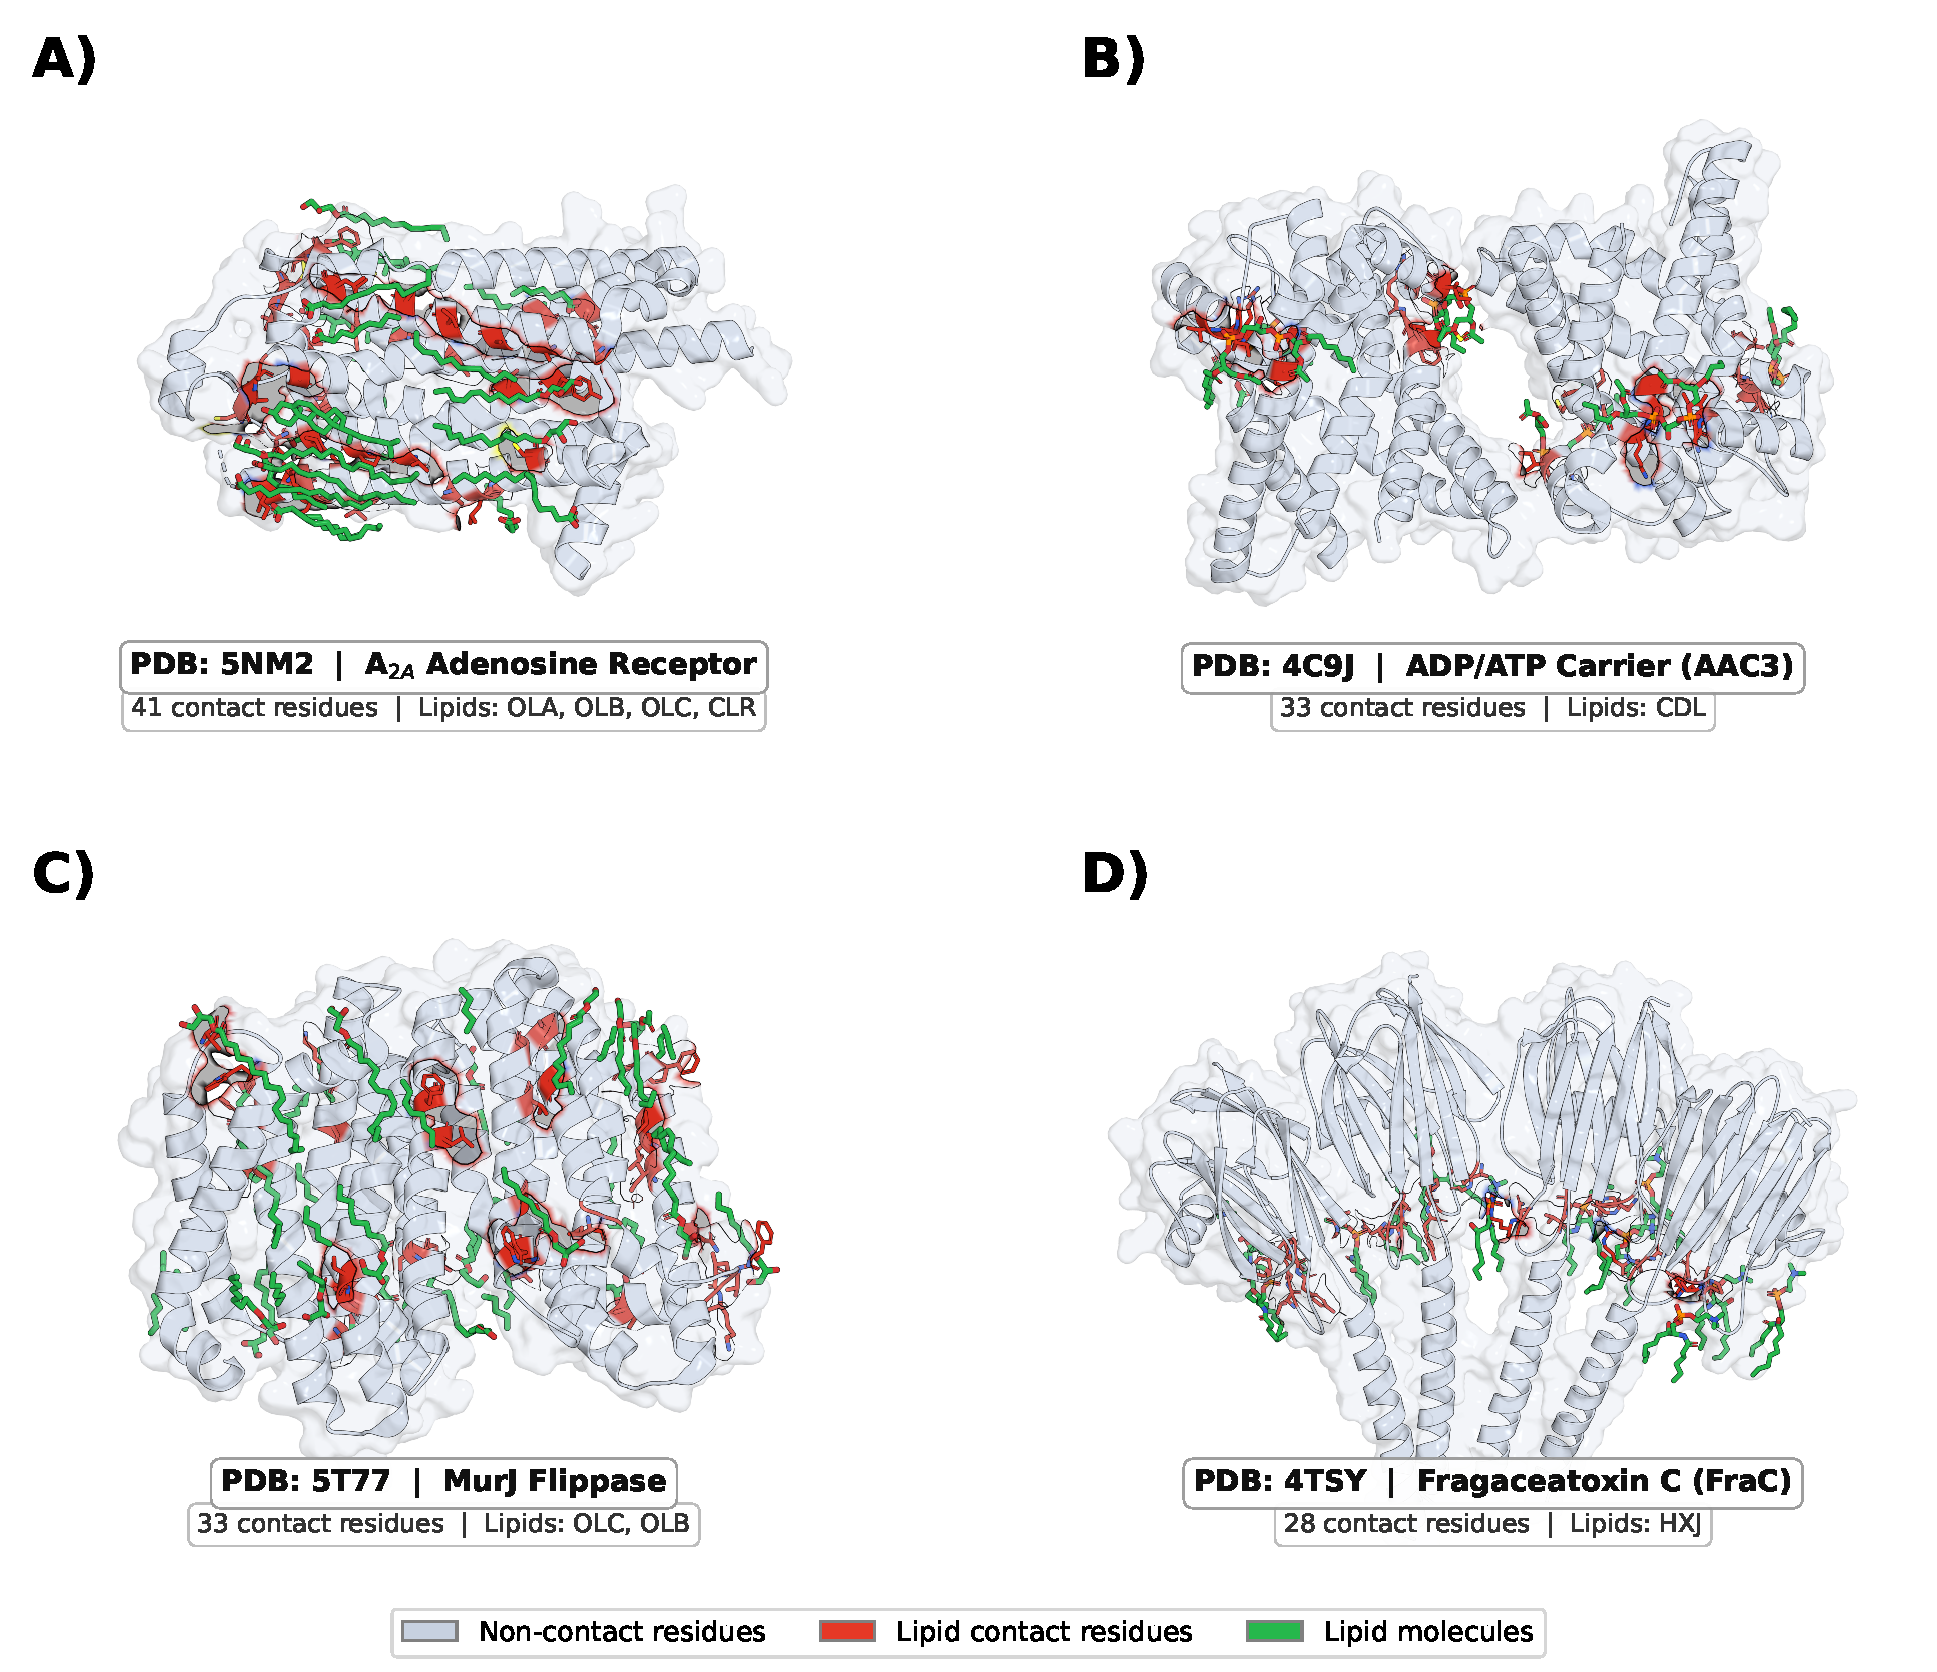
\includegraphics[width=\textwidth]{fig7_structural_visualization.pdf}
\caption{Structural visualization of MPLID lipid contact annotations across four representative membrane protein classes. (A) A\textsubscript{2A} adenosine receptor (PDB: 5NM2), a GPCR with 41 contact residues and four lipid types (oleic acid, cholesterol). (B) ADP/ATP carrier AAC3 (PDB: 4C9J), a mitochondrial transporter with 33 cardiolipin contact residues across two chains. (C) MurJ flippase (PDB: 5T77), a lipid II flippase with 33 contacts distributed across its transmembrane helices. (D) Fragaceatoxin C (PDB: 4TSY), a tetrameric pore-forming toxin with 28 sphingolipid contacts at the membrane insertion interface. These examples demonstrate that lipid contacts are site-specific rather than uniformly distributed across membrane-exposed surfaces.}
\label{fig:structures}
\end{figure*}


% ============================================================
\section{Methods}
% ============================================================

\subsection{Data source integration}

MPLID was constructed using a purely experimental approach with no dependence on computational membrane positioning databases. OPM data were not used at any stage of the MPLID construction pipeline; OPM is discussed in this paper solely to contextualize the complementary biological questions of membrane zone positioning versus direct lipid contact annotation. All residue annotations in MPLID derive exclusively from experimentally resolved lipid molecules in PDB structures. The RCSB Protein Data Bank \cite{berman2000, burley2023} was queried programmatically for all structures containing recognized lipid chemical components, identifying 8,221 candidate structures with lipid ligands. This query-first strategy ensures that every protein in the dataset has at least one experimentally resolved lipid molecule, providing an unbiased sampling of protein-lipid interactions across all structural classes. The identified structures were downloaded and processed through the contact calculation and quality filtering pipeline (Figure~\ref{fig:cluster}).

\subsection{Lipid molecule identification}

Lipid molecules in PDB structures were identified using their Chemical Component Dictionary codes. We compiled a list of 117 lipid codes organized into ten functional categories: phospholipids (CDL, POV, PCW, PEE, PGV, and others), cardiolipin (CDL, C9V, 18W, LCL), sphingolipids (SPH, S1P, HXJ, CRT), sterols (CLR, CHD, Y01, ERG), fatty acids (PLM, MYR, OLA, STE, ARA, DHA), glycerolipids (TGL, DAG, MAG), detergent mimetics (LDA, LMT, BOG, OLC, DPC), lipid A components (LPA, KDO, 6LP), and CHARMM simulation nomenclature (POPC, POPE, POPG, and others commonly found in cryo-EM depositions). This list was developed iteratively by cross-referencing the PDB Chemical Component Dictionary with lipid classification databases and manually curating entries to exclude non-lipid small molecules that might share similar chemical codes. Detergent mimetics were included because they frequently occupy native lipid binding sites in membrane protein crystal structures and provide relevant information about lipid-protein interaction geometry \cite{lee2004}.

\subsection{Structure processing and contact calculation}

For each candidate protein, the original PDB coordinate file was downloaded from RCSB to preserve HETATM records containing lipid molecule coordinates. Structure parsing was performed using BioPython \cite{cock2009}, extracting all standard amino acid residues (ATOM records) and all recognized lipid molecules (HETATM records). Non-standard residues, water molecules, metal ions, and non-lipid ligands were excluded.

Lipid contacts were defined using an all-atom distance criterion. For each protein residue $R$ and each lipid molecule $L$ in the structure, the minimum distance $d_{\min}(R, L)$ between any heavy (non-hydrogen) atom of $R$ and any heavy atom of $L$ was calculated. A residue was labeled as a lipid contact if:

\begin{equation}
d_{\min}(R, L) = \min_{a \in R,\, b \in L} \| \mathbf{r}_a - \mathbf{r}_b \| \leq 4.0~\text{\AA}
\label{eq:contact}
\end{equation}

\noindent where $\mathbf{r}_a$ denotes the Cartesian coordinates of heavy atom $a$ in residue $R$ and $\mathbf{r}_b$ denotes the coordinates of heavy atom $b$ in lipid $L$. The use of all heavy atoms (backbone and side chain) as residue representatives captures direct van der Waals contacts that would be missed by a C$\alpha$-only criterion, particularly for residues whose side chains extend into lipid-binding pockets while their backbone remains distant from lipid molecules. The 4.0~\AA{} cutoff was chosen to capture van der Waals contacts, consistent with standard distance thresholds in protein-ligand interaction analysis. For each residue, the minimum all-atom distance to the nearest lipid heavy atom was recorded regardless of contact status, providing a continuous distance metric that enables researchers to evaluate alternative cutoff values.

\subsection{Quality filtering}

Of the 8,221 candidate structures initially identified via RCSB queries, 9,796 PDB files were downloaded (including structures with multiple lipid types). After processing, 5,723 proteins yielded parseable structures. Of these, 1,011 were removed because they contained only non-lipid molecules misannotated as lipids (such as HEPES buffer and bacteriochlorophyll) or had all lipid atoms beyond the 4.0~\AA{} contact threshold, leaving 4,712 proteins with at least one genuine lipid contact. After sequence clustering and split assignment, the final dataset contains 4,704 proteins. This filtering ensures that every protein in the dataset has genuine, experimentally resolved lipid contacts.

\subsection{Sequence clustering}

To prevent data leakage between training, validation, and test splits, all 4,704 proteins were clustered using MMseqs2 \cite{steinegger2017} with a 30\% sequence identity threshold and 80\% bidirectional alignment coverage. These stringent thresholds ensure that proteins assigned to different splits are sufficiently divergent in sequence to represent independent test cases. The clustering produced 813 clusters.

\begin{figure*}[tbp]
\centering
\includegraphics[width=\textwidth]{fig6_cluster_analysis.pdf}
\caption{Sequence cluster analysis. (A) Distribution of cluster sizes at 30\% sequence identity on a log scale, showing a highly skewed size distribution with many singletons and a small number of large clusters containing many homologous structures. (B) Cumulative protein coverage ranked by cluster size, illustrating the concentration of proteins in a few large families.}
\label{fig:cluster}
\end{figure*}

\subsection{Split strategy}

Clusters were assigned to training, validation, and test splits using stratified random sampling at the cluster level, with stratification based on the average contact rate per cluster. This approach ensures that each split contains a representative distribution of high-contact and low-contact proteins. Entire clusters were assigned to a single split, guaranteeing that no two proteins sharing more than 30\% sequence identity appear in different partitions. The resulting splits contain 2,578 training proteins (54.8\%), 1,051 validation proteins (22.3\%), and 1,075 test proteins (22.9\%).

\subsection{Software and computational environment}

The MPLID construction pipeline was implemented in Python 3.11.8 using BioPython 1.83 \cite{cock2009} for PDB structure parsing, pandas 2.2.2 \cite{mckinney2010} for data manipulation, NumPy 1.26.4 for numerical computation, SciPy 1.13 for distance calculations, and scikit-learn 1.7.2 \cite{pedregosa2011} for data splitting. MMseqs2 version 15 \cite{steinegger2017} was used for sequence clustering. The RCSB PDB search API was used for programmatic identification of structures containing lipid chemical components.


% ============================================================
\section{Limitations}
% ============================================================

Several limitations should be noted when using MPLID. First, lipid contact labels depend on the crystallographic or cryo-EM resolution and completeness of resolved lipid molecules; many native lipid binding events are not captured because lipids are disordered or stripped during purification and crystallization. Consequently, the false negative rate is likely substantial, and the true positive rate of lipid contacts in membrane proteins is probably higher than the 1.00\% observed in MPLID. Moreover, many structures contain only one or a few resolved lipid molecules, meaning that the observed contacts represent a sparse snapshot of the full lipid-binding landscape rather than a comprehensive map of all possible interaction sites. Second, the inclusion of detergent mimetics as proxy lipids introduces potential noise, as detergent binding sites may not perfectly recapitulate native lipid interactions. Analysis of HETATM records across all processed PDB files shows that approximately 17\% of proteins with recognized lipid molecules contain exclusively detergent mimetics (e.g., dodecyl maltoside, octyl glucoside, lauryldimethylamine oxide) without any physiological lipid species, while an additional 10\% contain both detergent and physiological lipids. This means that for roughly one in six proteins, all contact labels derive from crystallization detergents rather than native lipid species. Third, the dataset inherits biases from the PDB toward well-studied, readily crystallizable membrane protein families, leaving many therapeutically relevant but structurally uncharacterized families underrepresented. Finally, the 4.0~\AA{} distance cutoff is a single threshold that may not be optimal for all lipid types; researchers are encouraged to explore alternative cutoffs using the continuous distance values provided in the dataset. Additionally, because MPLID annotations are derived from static crystallographic and cryo-EM snapshots, they may not fully represent the dynamic nature of protein--lipid interactions in native membrane environments, where lipids undergo lateral diffusion and exchange on nanosecond-to-microsecond timescales. Crystal packing artifacts may also contribute false positive contacts, as lipid molecules resolved in crystal structures can occupy lattice contact interfaces that do not reflect native membrane binding.

No structure resolution cutoff was applied during dataset construction: all PDB structures with recognized lipid molecules were included regardless of crystallographic resolution. While this maximizes dataset size, low-resolution structures (worse than 3.5~\AA{}) may have less reliable lipid positions, potentially introducing noise into contact labels. Researchers working with resolution-sensitive applications are encouraged to filter by PDB resolution using the provided \texttt{pdb\_id} field.

The current release does not include per-residue lipid chemical component codes, meaning that users cannot directly determine which lipid type (e.g., cholesterol versus cardiolipin) contacts a given residue. However, the continuous \texttt{min\_distance} values enable evaluation of alternative distance cutoffs, and the \texttt{pdb\_id} field allows users to retrieve lipid identities from the original PDB structures. Lipid type stratification at the residue level is planned for a future release.

Four selenocysteine (SEC) residues in the dataset are all annotated as lipid contacts (4/4, 100\% contact rate). Given the extremely small sample size, this observation is not statistically meaningful and these residues were excluded from enrichment ratio analysis.

Cross-validation of MPLID labels against the curated dataset used by the DREAMM prediction method \cite{chatzigoulas2022} is planned as future work to assess concordance between the two independently derived annotation approaches.

MPLID is intended as a ground-truth resource for residue-level lipid contact annotation and does not aim, by itself, to provide an optimized predictive solution to the full experimental-only classification problem.


% ============================================================
\section{Re-use Potential}
% ============================================================

MPLID is designed to serve as a large-scale training and evaluation resource for multiple research applications in structural bioinformatics, drug discovery, and membrane biology.

\subsection{Machine learning for lipid contact prediction}

The principal application of MPLID is as a training and evaluation dataset for developing machine learning models that predict lipid contact residues from protein sequence or structure. The pre-defined, cluster-aware train/validation/test splits enable standardized model comparison, and the class imbalance (1.00\% positive rate, approximately 100:1 negative-to-positive ratio) presents a realistic and challenging binary classification task that requires specialized approaches such as class weighting, oversampling (SMOTE) \cite{chawla2002}, or focal loss functions. The scale of the dataset is sufficient for training deep neural networks, including architectures that combine structural descriptors with protein language model embeddings from ESM-2 \cite{lin2023} or ProtTrans \cite{elnaggar2022}. We note that the Matthews correlation coefficient should be used as the primary evaluation metric for this task due to the substantial class imbalance, as accuracy and even F1 scores can be misleading when the negative class dominates.

\subsection{Drug discovery applications}

Lipid binding sites on membrane proteins represent an emerging class of druggable targets. General anesthetics, neurosteroids, and endocannabinoids modulate ion channels and GPCRs through specific lipid binding sites \cite{duncan2020, brannigan2008}, and cholesterol binding sites on GPCRs are increasingly recognized as allosteric modulatory sites \cite{hanson2008, fantini2013}. MPLID can inform the identification of lipid-mimetic drug binding sites by providing a catalog of experimentally validated lipid interaction residues across thousands of membrane proteins. Predicted lipid contact sites on therapeutically relevant proteins can guide the design of lipid-conjugated prodrugs, membrane-anchored therapeutics, or allosteric modulators that exploit lipid binding pockets.

\subsection{Structural biology and protein engineering}

Understanding which residues contact lipids is essential for rational membrane protein engineering. Mutations at lipid contact sites can destabilize membrane proteins, alter their trafficking, or modify their functional properties. MPLID provides data to train models that predict which residues are critical for lipid-mediated stability, enabling more informed design of stabilizing mutations for membrane protein crystallization, cryo-EM, or functional studies. Additionally, the dataset supports comparative analysis of lipid contact patterns across protein families, enabling identification of conserved lipid binding motifs and family-specific interaction signatures. Future work incorporating cavity-based structural analysis could further support the observation that many residues located within the membrane region do not form direct lipid contacts, reinforcing the conceptual separation between membrane localization and residue-level interaction. These interpretations are based on static structural snapshots. Incorporation of dynamic information may alter residue--lipid proximity patterns, as conformational fluctuations could transiently modify contact definitions.

\subsection{Computational label comparison studies}

The availability of MPLID alongside OPM membrane zone annotations enables systematic comparison of experimental lipid contacts with computational membrane boundaries. We compared MPLID contact labels with OPM-derived membrane zone assignments across proteins present in both resources (Figure~\ref{fig:opm_comparison}). The number of overlapping proteins varies by analysis: 2,383 proteins contributed to precision estimates, 1,685 to recall estimates, and 2,457 to contact distribution analysis, reflecting differences in the availability of OPM membrane zone annotations and non-zero lipid contacts across the shared set. Of all MPLID lipid contacts in the shared set ($n = 28{,}497$ residues), 51.2\% fell within the OPM membrane zone while 48.8\% were located outside the computationally defined boundaries, likely reflecting interfacial contacts, re-entrant loops, or amphipathic helices that extend beyond the hydrophobic core. Conversely, 98.8\% of OPM membrane zone residues ($n = 1{,}170{,}590$) showed no direct lipid contact within 4.0~\AA{}, and the per-protein median was only 0.7\% of membrane zone residues having lipid contacts. The OPM membrane zone captured a median of 50.0\% of lipid contacts per protein. These dataset-wide statistics highlight the fundamental difference between membrane zone classification and lipid contact prediction: being embedded in the membrane is neither sufficient nor necessary for direct lipid interaction. Researchers working with MemProtMD \cite{newport2019} simulations can similarly compare simulated lipid contacts with the experimental contacts provided by MPLID.

\begin{figure*}[tbp]
\centering
\includegraphics[width=\textwidth]{fig8_opm_comparison.pdf}
\caption{Quantitative comparison of MPLID lipid contacts versus OPM membrane zone annotations. (A) Residue classification overlap: 48.8\% of lipid contacts ($n = 28{,}497$) fall outside the OPM membrane zone, while 98.8\% of OPM zone residues ($n = 1{,}170{,}590$) lack direct lipid contact. (B) Per-protein OPM precision ($n = 2{,}383$ proteins): median 0.7\% of membrane zone residues have lipid contacts. (C) Per-protein OPM recall ($n = 1{,}685$ proteins): the membrane zone captures a median of 50.0\% of lipid contacts. (D) Per-protein scatter of contacts inside versus outside the OPM zone ($n = 2{,}457$ proteins). These results demonstrate that membrane zone classification and lipid contact annotation address fundamentally different biological questions.}
\label{fig:opm_comparison}
\end{figure*}

\subsection{Integration with protein language models}

The residue-level format of MPLID is directly compatible with per-residue embeddings from protein language models. Each residue's 1,280-dimensional ESM-2 embedding \cite{lin2023} or 1,024-dimensional ProtTrans embedding \cite{elnaggar2022} can be concatenated with structural descriptors and used as input to supervised classifiers. The 813 sequence clusters provide sufficient diversity to evaluate whether language model representations generalize across membrane protein families with limited sequence similarity. Alternatively, MPLID can be combined with interpretable structural descriptor frameworks, such as STING RDB-derived nanoenvironment descriptors \cite{neshich2003, neshich2006}. In this setting, residue-level lipid contacts may be analyzed in terms of explicit physicochemical and geometric properties, enabling mechanistic interpretation of the nanoenvironment characteristics associated with lipid interaction. This dual compatibility supports both high-capacity representation learning approaches and descriptor-based, interpretable modeling strategies.


% ============================================================
\section{Availability of supporting source code and data}
% ============================================================

The complete MPLID dataset is deposited at Zenodo under a CC0 public domain dedication with persistent DOI: \url{https://doi.org/10.5281/zenodo.18487584} \cite{zenodo_mplid}. Upon acceptance, the dataset will also be deposited in GigaDB in accordance with journal policy. The Zenodo archive contains the full residue-level annotations (train, validation, and test splits as gzip-compressed CSV files), protein-level metadata, amino acid composition statistics, and a data dictionary describing all fields.

All code for reproducing the dataset from raw PDB structures is available in a public GitHub repository: \url{https://github.com/omagebright/MPLID}. The repository includes the complete processing pipeline (structure downloading, lipid identification, contact calculation, quality filtering, and split generation), analysis scripts for generating figures and tables, and documentation of the data schema and methodology.

The dataset and code are organized following FAIR principles \cite{wilkinson2016}: data are Findable via persistent DOIs and indexed metadata; Accessible through standard HTTPS download from Zenodo and GitHub; Interoperable using standard CSV format with documented column definitions; and Reusable under permissive open licenses (CC0 for data, MIT for code).


% ============================================================
\section{Conflicts of interest}
% ============================================================

The authors declare that they have no competing interests.


% ============================================================
\section{Funding}
% ============================================================

This research was funded by the S\~{a}o Paulo Research Foundation (FAPESP) (grant nos. 2023/02691-2, 2025/23708-6).


% ============================================================
\section{Data availability}
% ============================================================

The data underlying this article are available in Zenodo at \url{https://doi.org/10.5281/zenodo.18487584}, and in a public GitHub repository at \url{https://github.com/omagebright/MPLID}.


% ============================================================
\section{Author contributions statement}
% ============================================================

Author contributions follow the CRediT taxonomy. F.B.O.: Conceptualization, Methodology, Software, Formal Analysis, Data Curation, Writing (Original Draft), Visualization. G.N.: Conceptualization (dataset definition and biological framework), Supervision, Writing (Original Draft, Review \& Editing), Funding Acquisition. Both authors read and approved the final manuscript.


% ============================================================
\section{Ethics approval and consent to participate}
% ============================================================

Not applicable. This study uses publicly available structural data from the Protein Data Bank and does not involve human subjects, animal experiments, or clinical data.



% ============================================================
\section{Acknowledgments}
% ============================================================

The authors thank Ivan Mazoni and In\'{a}cio Henrique Yano for their contributions to data validation and resource management during the early stages of this work. The authors thank Embrapa Digital Agriculture (Embrapa Agricultura Digital) for computational resources and infrastructure support. The authors acknowledge the RCSB Protein Data Bank \cite{berman2000, burley2023} and the OPM database \cite{lomize2012} teams for maintaining the essential structural biology resources upon which this work depends. The authors thank the developers of MMseqs2 \cite{steinegger2017}, BioPython \cite{cock2009}, and the broader open-source scientific computing community for the software tools used in this study.



% ============================================================
\section{Abbreviations}
% ============================================================

\noindent
\textbf{MPLID}: Membrane Protein-Lipid Interaction Database;
\textbf{PDB}: Protein Data Bank;
\textbf{OPM}: Orientations of Proteins in Membranes;
\textbf{GPCR}: G protein-coupled receptor;
\textbf{MCC}: Matthews correlation coefficient;
\textbf{CG-MD}: Coarse-grained molecular dynamics;
\textbf{FAIR}: Findable, Accessible, Interoperable, Reusable;
\textbf{CDL}: Cardiolipin;
\textbf{CLR}: Cholesterol;
\textbf{PLM}: Palmitic acid;
\textbf{DREAMM}: Detection of Residues on Exposed Areas of Membrane-associated Macromolecules;
\textbf{ESM-2}: Evolutionary Scale Modeling 2;
\textbf{SMOTE}: Synthetic Minority Over-sampling Technique;
\textbf{RCSB}: Research Collaboratory for Structural Bioinformatics;
\textbf{CSV}: Comma-separated values.


% ============================================================
% References
% ============================================================

\bibliographystyle{unsrtnat}
\bibliography{references}

\end{document}
